The majority of the theoretical background in this work will hinge almost in its entirety on the validity of the equations \eqref{eq:divergence_curl}, and theory sufficient for understanding their applications will be discussed in this section.
\begin{definition}[Pseudo-\textsc{Riemann} manifold]
  An $n$-dimensional manifold \gls{manifold} is a topological space locally similar to Euclidean space $\mathbb{E}^n$, in  a smooth sense.
  It is said to be of the pseudo-\textsc{Riemann} kind if it is equipped with the non-degenerate \textsc{Riemann} metric $\mathfrak{g}$.
\end{definition}
\noindent The \textsc{Riemann} metric is left purposefully unspecified, as it depends on the representation of the manifold chosen.
Throughout this work, we shall work the pesudo-\textsc{Riemann} manifold $\Omega$ of dimension 3, but we shall for the moment consider one of dimension $n$ so as to speak of the details in general.
The intrinsic smoothness of the manifold reveals something about its differentiability, which is defined by the tangent space of some point in the manifold, $\Tangent_p\Omega$.
A tangent space $\Tangent_p\Omega$ is technically a local space containing all tangent vectors at some point $p \in \Omega$,\footnote{\cite{flanders1989differential} \textsc{Flanders}, p.54} so we shall introduce the \emph{tangent bundle} as the disjoint union of such spaces for all points on the manifold, $\gls{tangent-bundle} = \sqcup_p\Tangent_p\Omega$,\footnote{\cite{jost2011riemannian} \textsc{Jost}, p.12} equipped with a natural projection $\Pi \colon \Tangent\Omega\to\Omega$, such that vector fields $\uvec \in \Tangent_p\Omega$ are mapped to $\Pi(\uvec) = p$.\footnote{\cite{morita2001geometry} \textsc{Morita}, pp.169--171}
Defining an inner product on this space, $\langle \avec, \bvec \rangle = [\mathfrak{g}]_{ij} a^{i} b^{j}$, where \textsc{Einstein} summation is implied, induces the metric.

In order to construct a meaningful notion of operations on the tangent bundle, we endow its dual, the cotangent bundle \gls{cotangent-bundle}, the exterior product \gls{exterior-product}, forming the exterior algebra \gls{exterior-algebra}.
The exterior product may appear obtuse when first presented in the abstract manner we will shortly do, but rest assured it does indeed have a geometric interpretation.
For, in an effort to unite the exterior algebra of Hermann \textsc{Grassmann}\footnote{\cite{grassmann1878lineale} \textsc{Grassmann}, \S55} and the quaternion algebra of William Rowan \textsc{Hamilton},\footnote{\cite{hamilton1844quaternions} \textsc{Hamilton} (1844)} William Kingdon \textsc{Clifford} laid the foundation on which the theory of the nominal \textsc{Clifford} algebras were built.\footnote{\cite{clifford1878applications} \textsc{Clifford} (1878)}
On such algebras, the exterior product of $k$ covectors is understood to be the oriented volume of the $k$-paralellotope bound by them,\footnote{\cite{grassmann1878lineale} \textsc{Grassmann}, pp.50--51} and is just one part of the so-called \emph{geometric product}, which provides a coherent definition of a vector product in general.
We shall only draw from this intuition at a later point, as we shall focus on the properties of the exterior product with respect to objects on sections of the cotangent bundle.

Labeling the projection of a covector field $\ufrak \in \Tangent^{\ast}\Omega$ in the same manner as a vector field, $\Pi^{\ast}(\ufrak) = p$, we define the section to be its inverse operation, uniquely returning the point to the covector field.
The repeated application of the exterior product however admits higher grade covector fields.
We will therefore use for a grade $k$ monomial section of the exterior algebra $\afrak \in \Lambda^{k}\Omega$ a $k$-form, and avoid the terminology of covectors altogether, as forms serve a much broader purpose to our end.
The exterior product is alternating in the sense that for $\afrak_i \in \Lambda\Omega$, given a permutation $\sigma$ of the positive integers up to $k$, we have $\afrak_{\sigma(1)}\wedge\cdots\wedge\afrak_{\sigma(k)} = \signum{(\sigma)} \, \big( \afrak_{1}\wedge\cdots\wedge\afrak_{k} \big)$.
The sign of a permutation $\signum(\sigma)$ is $1$ if the number of transpositions from the identity permutation is even, and $-1$ if the number of transpositions is odd.
This alternating property further reduces to the two properties that
\begin{subequations}\label{eq:exterior_product}
        \begin{equation}\tag{\theequation{a, b}}
                \afrak\wedge\afrak \equiv 0, \qquad \afrak\wedge\bfrak \equiv -\bfrak\wedge\afrak,
        \end{equation}
\end{subequations}
for any forms $\afrak, \bfrak$, of the same or different grade.
To summarize, then:
\begin{definition}[Exterior algebra]
  Let $\Tangent\Omega$ be a tangent bundle with basis $\partial_i$, and let $\wedge$ denote the product of the algebra $\Lambda\Omega = \Tangent^{\ast}\Omega$.
  Then the members of the algebra
  \[
        \dee x^{i} = {\Big( {[\mathfrak{g}]}^{ij}\partial_{j} \Big)}^{\flat}
  \]
  form a basis for the cotangent bundle.
  When $\wedge: \Lambda^{k}\Omega \times \Lambda^{l}\Omega \to \Lambda^{k + l}\Omega$ satisfies the conditions of bilinearity and associativity, in addition to the modified alternating condition of equation \subeqref{\ref{eq:exterior_product}}[b]
  \begin{equation}
    \afrak \wedge \bfrak = {(-1)}^{kl} \bfrak \wedge \afrak,
  \end{equation}
  it is an exterior product, and $\Lambda^{k + l}\Omega$ is an exterior algebra.
\end{definition}
\noindent Vector fields, then, as far as this work is concerned, are sections of the tangent space, though we will not notationally distinguish them.
The notion of a tangent space is inherently connected to some sense of differentiability.
Thus, given a differentiable curve on the manifold, the tangent vector at a point is described by this differentiability, and the partial derivative operators form a basis for the tangent space with respect to local coordinates on the manifold.
We may choose for it some local basis $\{ \evec_j \}$, such that a vector field may be expressed $\uvec = u^{j}\evec_{j}$.
For $\mathbb{E}^3$, with coordinates $x,y,z$ specifically, we shall always write its basis as $\{ \partial_x, \partial_y, \partial_z \} \simeq \{ \ihat, \jhat, \khat \}$.
This \emph{dual space} we discussed earlier may be regarded as the space of all linear functionals from the tangent space onto the field over which the vector field lies.
Consider still the general basis vectors $\evec_j$, along with some dual basis $\{ \evec^{i} \}$.
As a result of the above discussion, we must have that $\evec^{i}(\evec_{j}) = \delta_{j}^{i}$.
Clearly,
\[
  \evec^{i}(\uvec) = \evec^{i}(u^j \evec_j) = u^j \evec^{i} \evec_{j} = u^j \delta_{j}^{i} = u^i.
\]
In fact, any $k$-form is by construction a functional over the space of vector fields on the manifold.
It is clear that there exists some isomorphism between the vectors and covectors.
If $\ufrak \in \Lambda\Omega$ and $\uvec \in \Tangent\Omega$ are isomorphic, these isomorphisms are usually denoted by the sharp $\ufrak^{\sharp} = \uvec$ and the flat $\uvec^{\flat} = \ufrak$, respectively raising and lowering the indices of the coefficients.\footnote{\cite{nishikawa2002variational} \textsc{Nishikawa}, \S3.1}
Stated explicitly, with these operators, we may describe any vector field $\uvec = u\ihat + v\jhat + w\khat$ in terms of differential forms as ${\uvec}^{\flat} = u\,\dee x + v\,\dee y + w\,\dee z$, so that $u^{i} \partial_i \simeq u_{i}\,\dee x^{i}$.
This notation however tends to clutter expressions and is cumbersome to read, and it will only be used when strictly necessary.
As the astute reader may have noticed, we already readily distinguish between elements of the cotangent and tangent spaces by denoting the former with a fraktur typeface, and the latter with an italic bold.
Thus it should be clear from context whichever of the two is meant at any given time.

We note the above expression implies the basis covectors, and indeed reiterate the fact that $k$-forms themselves are functions of vectors fields.
In fact, when $\afrak\in\Lambda\Omega$, we have that $\afrak(\uvec) = a_i u^j$, which is a zero-form, or scalar.
This generalizes to higher grade forms, with the introduction of the interior product, acting as a contraction in the usual sense of the term.
\begin{definition}[Interior product]
  Let $\uvec \in \Tangent\Omega$, and $\afrak\wedge\bfrak \in \Lambda^{k+l}\Omega$, noting the order of the addition of exponents in the exterior algebra.
  The interior product $\iprod: \Tangent\Omega \times \Lambda^{k + l}\Omega \to \Lambda^{k + l - 1}$, is given by
  \[
        \uvec\iprod(\afrak\wedge\bfrak) = (\uvec\iprod\afrak)\wedge\bfrak + {(-1)}^{k}\afrak\wedge\uvec\iprod\bfrak.
  \]
  For unit $\bfrak$, we have $\afrak \wedge 1 = \afrak$, and so we say $\uvec \iprod \afrak = \afrak(\uvec)$.
\end{definition}

\noindent Extrapolating on this idea that the tangent space is inherently dependent on some notion of differentiability forming a basis for the tangent space, the cotangent space must then have a corresponding operation, which we will label the exterior derivative.
\begin{definition}[Exterior derivative]
  Given a manifold $\Omega$ and basis $\{ \partial_{i}\}$, the exterior derivative $\dee \colon \Lambda^k \Omega \to \Lambda^{k+1} \Omega$ of a $k$-form $\afrak = a_{\mathcal{i}}\,\dee x^{\mathcal{i}}$ is given by $\gls{exterior-derivative} = \partial_{i} a_{\mathcal{i}} \,\dee x^{i} \wedge \dee x^{\mathcal{i}}$, where $\mathcal{i}$ is a multi-index of $i$.
  The product rule is graded, namely $\dee(\afrak\wedge\bfrak) = \dee\afrak\wedge\bfrak + {(-1)}^k \afrak\wedge\dee\bfrak$.
  Furthermore, $\dee\dee\afrak \equiv 0$.
\end{definition}
\noindent In the manipulation of expressions of forms, it shall be necessary to convert forms of a higher grade to one of lower grade, and \emph{vice versa}, for example before or after computing the exterior derivative.
To that end, we introduce the \textsc{Hodge} star-operator.
\begin{definition}[\textsc{Hodge} operator]
  The \textsc{Hodge} operator $\gls{hodge-star}: \Lambda^{k}\Omega \to \Lambda^{n-k}\Omega$, where $n$ is the dimension of $\Omega$, such that $\afrak \wedge \star\bfrak = \langle \afrak, \bfrak \rangle \,\dee V$.
  It holds that $\star\star\afrak = {(-1)}^{k(n-k)}\afrak$.
\end{definition}

\noindent With the exterior derivative, we may describe the volume of the space with respect to local coordinates.
In particular, for a manifold $\Omega$ of dimension $n$, $\dee V \equiv \sqrt{\absl{\mathfrak{g}}} \dee x^{1} \wedge \cdots \wedge \dee x^{n}$, where $\absl{\mathfrak{g}}$ is the determinant of the local metric.
We find from the definition of the \textsc{Hodge} star above that $\star\dee V = 1$.

In order to study the exterior derivative under the \textsc{Hodge} operator, we define the \emph{codifferential}, given as follows.\footnote{\cite{morita2001geometry} \textsc{Morita}, \S4.2}
\begin{definition}[Coderivative]
  The codifferential of a $k$-form is adjoint to the exterior derivative, and is given by
  \[
        \gls{coderivative} = {(-1)}^{k} \star^{-1} \dee \star \afrak = {(-1)}^{n(k+1) + 1} \star \dee \star \afrak.
  \]
\end{definition}

\noindent For illustrative purposes, the relationship between the exterior derivative, coderivative, and \textsc{Hodge} star is given by the following commutative diagram.
\begin{figure}[H]
  \centering
  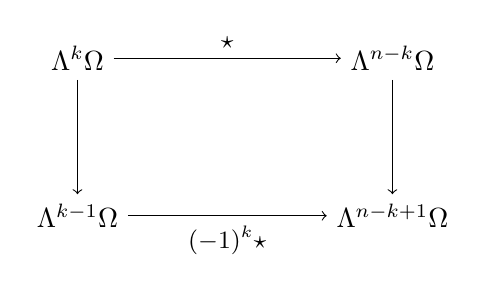
\begin{tikzpicture}
    \begin{scope}[scale = 2]
      \node (A) at (0,1) {$\Lambda^{k}\Omega$};
      \node (B) at (2,1) {$\Lambda^{n-k}\Omega$};
      \node (C) at (0,0) {$\Lambda^{k-1}\Omega$};
      \node (D) at (2,0) {$\Lambda^{n-k+1}\Omega$};
      \draw[->, font = \small] (A.east)--(B.west) node[midway, above]{$\star$};
      \draw[->, font = \small] (A.south)--(C.north) node[midway, left]{$\codee$};
      \draw[->, font = \small] (B.south)--(D.north) node[midway, right]{$\dee$};
      \draw[->, font = \small] (C.east)--(D.west) node[midway,below]{${(-1)}^{k}\star$};
    \end{scope}
  \end{tikzpicture}
\end{figure}

\noindent As we have noted, we are strictly speakning not performing these operations on the space $\Lambda^{k}\Omega$, but rather sections of it.
On these sections we may define an inner product that should be familiar,
\begin{equation}\label{eq:L2-norm}
        (\afrak, \bfrak) = \int_{\Omega} \langle \afrak, \bfrak \rangle \,\dee V = \int_{\Omega} \afrak \wedge \star \bfrak.
\end{equation}
We have of course not defined what the integral of a differential form actually is.
Still, assuming inheritance from our familiar notion of the integral as a linear operator, we find that it does indeed constitute an integral analogous to that of the $L^2$ inner product.
This inner product is symmetric, and is the inner product with respect to which the codifferential is adjoint to the exterior derivative, in the sense that $( \dee\afrak, \bfrak ) = ( \afrak, \codee\bfrak )$.
For proofs and further discussion on the codifferential operator, the reader is again refered to \textsc{Morita}'s monograph.\footnote{\cite{morita2001geometry} \textsc{Morita}, pp.153--155}

We are now nearing the revelation of the fundamental theorem of multivariate calculus, and with it the end of this section.
Before this, however, we ought to finally apply the operators to these differential forms to get a sense of the reason for which they were introduced to begin with.
Consider the Euclidean vector field $\uvec^{\flat} = u\,\dee x + v\,\dee y + w\dee z$.
Upon calculating its exterior derivative $\dee\ufrak$, one finds that
\[
        \dee\ufrak = \big( \deex v - \deey u \big)\,\dee x \wedge \dee y + \big( \deez u - \deex w \big)\,\dee z \wedge \dee x + \big( \deey w - \deez v \big)\,\dee y \wedge \dee z.
\]
This is nothing less than the two-form corresponding to the curl.
Furthermore, the coderivative of a vector field is given by $\codee\ufrak = -{\star}\dee{\star}\ufrak$, which upon calculation one finds to be
  \[
        \codee\ufrak = -\big(\deex u + \deey v + \deez w \big).
  \]
This is of course the divergence with an opposite sign.
And so, we define the operators to be such.

\begin{definition}[Curl and divergence]
  Let $\ufrak \in \Lambda^{k}\Omega$, with $\dim\Omega = 3$.
  The curl and divergence of $\ufrak$ are respectively given by
  \[
        \Curl{\ufrak} = \star\dee\ufrak, \qquad \Div{\ufrak} = \star\dee{\star}\ufrak.
  \]
\end{definition}

\noindent From these definitions, it is trivial to prove identities of great utility.
For example, $\Div\Curl\ufrak$ and $\Curl\Grad\ufrak$ both being identically equal to zero.
Another way to express the divergence is to consider the contraction of the gradient.
We understand the trace of a matrix to be a form of contraction,\footnote{expand on this.} and the divergence of a vector field is simply the trace of the gradient.\footnote{confirm this.}
For brevity, we take an \emph{ad hoc} approach.
Consider the exterior derivative of the interior product $\uvec\iprod\dee V$.
We calculate that
\begin{equation}\label{eq:exterior_divergence}
        \begin{aligned}
           \dee(\uvec\iprod\dee V) &= \dee\sum_{i} {(-1)}^{i+1} u_i \dee x^{1} \wedge \cdots \wedge \widehat{\dee x^{i}} \wedge \cdots \wedge \dee x^{n}\\
           &= \partial_i u_i \dee V \\
           &= \Div\uvec\,\dee V,
        \end{aligned}
\end{equation}
where $\widehat{\dee x^{i}}$ in the first equality in equation \eqref{eq:exterior_divergence} means the term is omitted.

Having an idea of what the divergence and curl actually are, we are now ready for the progenitor of their named theorems---the fundamental theorem of multivariate calculus.
The proof for this theorem is beyond the scope of the present work, so it will only be stated.

\begin{theorem}[Fundamental Theorem of Multivariate Calculus]
  Let $\ufrak \in \Lambda^{n-1}\Omega$, and $\partial\Omega$ be the sufficiently regular boundary of $\Omega$.
  Then,
  \begin{equation}\label{eq:ftmc}%FTMC - Fundamental Theorem of Multivariate Calculus
        \int_{\partial\Omega} \ufrak = \int_{\Omega} \dee\ufrak.
  \end{equation}
\end{theorem}

\noindent The convergence of integrals of the form \eqref{eq:ftmc} only makes sense for an unbounded fluid domain should the differential form $\ufrak$ evanesce sufficiently fast.
This is clear from the condition that $\ufrak$ shall have compact support, meaning it would need to be a distribution.
Such liberties are not ones we may always take, so we will make a concession in our definition of the manifold $\Omega$.
Suppose $\partial\Omega = S \cup \Sigma$, such that $\Sigma$ encloses $\Omega$, whilst $S$ excises it, as is shown in figure \ref{fig:manifold}.
We may now extend $\Sigma$ in such a way that $\Omega$ remains compact, and the general properties of $\ufrak$ are conserved, now only requiring sufficiently rapid evanescence.

\begin{figure}
  \centering
  \scalebox{1.25}{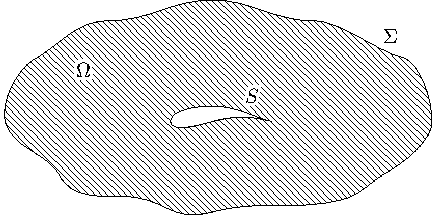
\includegraphics{manifold.pdf}}
  \caption{A cross section of $\Omega$, illustrating the boundaries $S\cup\Sigma = \partial\Omega$.}
  \label{fig:manifold}
\end{figure}
An interesting inquiry to propose is of course how a punctured manifold behaves differently than one which is not.
The answer is simple---problems will arise concerning the behavior of closed differential forms.
We consider the following.

\begin{lemma}[\textsc{Poincaré}]
  Let $\afrak \in \Lambda^k\mathbb{R}^n$ be an arbitrary closed form, meaning $\dee\afrak = 0$.
  There then exists a form $\bfrak \in \Lambda^{k-1}\mathbb{R}^n$ such that $\afrak = \dee\bfrak$.
\end{lemma}

\noindent The terminology for a form being the exterior derivative of some other form is \emph{exact}.
The \textsc{Poincaré} lemma states the manifold of figure \ref{fig:manifold}, we can always find some local representation such that any closed form is exact.


As was noted above, the \textsc{Gauss}--\textsc{Ostrogradsky} theorem of equation \subeqref{\ref{eq:divergence_curl}}[a] is a special case of equation \eqref{eq:ftmc}.
To show this, we recall the result of equation \eqref{eq:exterior_divergence}, and consider the following equality.
\[
        \int_{\Omega} \dee(\uvec\iprod\dee V) = \int_{\partial\Omega} \uvec\iprod\dee V.
\]
Indeed, $\uvec\cdot\nhat\dee S = u\,\dee y\wedge\dee z - v\,\dee z\wedge\dee x + w\,\dee x\wedge\dee y = \uvec\iprod\dee V$.
And with that, the major requisite of the boundary element method is proved---namely its progenitor.
It will be shown that the boundary element method applied to solenoidal fluid flow of no vorticity.

\begin{definition}[\textsc{Hodge}--\textsc{Laplace} operator]
  Let $\ufrak \in \Lambda^{k}\Omega$.
  We define the \textsc{Hodge} Laplacian to be
  \begin{equation}\label{eq:Hodge_laplacian}
    \Delta \ufrak = \codee \dee \ufrak + \dee \codee \ufrak.
  \end{equation}
  Should $\Delta \ufrak = 0$, then $\ufrak$ is said to be harmonic.
\end{definition}

Furthermore, we introduce a theorem of as great importance as the fundamental theorem of multivariate calculus.

\begin{theorem}[\textsc{Hodge} decomposition]\label{thm:Hodge_decomposition}
  Any differential form $\ufrak$ may be decomposed as $\dee \afrak + \codee \bfrak + \mathfrak{c}$, where $\Delta \mathfrak{c} = 0$.
\end{theorem}

\[
        \iota: \partial\Omega \righthook \Omega
\]
